\documentclass[12pt]{report}
\usepackage[utf8]{inputenc}
\usepackage{graphicx}
\graphicspath{{images/}}
\usepackage{multirow}
\usepackage{float}
\usepackage{subcaption}
\usepackage[a4paper, width=150mm, top=25mm, bottom=25mm]{geometry}
\usepackage{fancyhdr}
\usepackage{amsmath}
\usepackage{titlesec}
\usepackage{comment}
\usepackage{pythonhighlight}
\usepackage[numbers]{natbib}
\usepackage{hyperref}
\hypersetup{
    colorlinks=true,
    linkcolor=black,
    filecolor=magenta,      
    urlcolor=blue,
    citecolor=black,
    pdftitle={Overleaf Example},
    pdfpagemode=FullScreen,
    }
\usepackage{mathtools}

\newcommand\Myperm[2][^n]{\prescript{#1\mkern-2.5mu}{}P_{#2}}
\newcommand\Mycomb[2][^L]{\prescript{#1\mkern-0.5mu}{}C_{#2}}
\DeclarePairedDelimiter\ceil{\lceil}{\rceil}
\DeclarePairedDelimiter\floor{\lfloor}{\rfloor}

\titleformat{\chapter}[hang] 
{\normalfont\huge\bfseries}{\chaptertitlename\ \thechapter:}{1em}{}
\pagestyle{fancy}
\fancyhead{}
\fancyhead[L]{\thesection}
\fancyhead[R]{\textbf{Entropy using cellular automata}}
\fancyfoot{}
\fancyfoot[L]{\thepage}
\fancyfoot[R]{Bowen Shiro Husin}
\setlength\parindent{0pt}

\begin{document}
\begin{titlepage}
    \begin{center} 
       \vspace*{1cm}
       
       \textbf{ \LARGE A visual demonstration of Entropy}

       \vspace{6.5cm}
       \large{A simulation of random processes using cellular automata}.


       \vspace{7.0cm}
       \large{By: Bowen Shiro Husin} \par
       
       \vspace{0.3cm}
       25th February 2023

    
        
    \end{center}
\end{titlepage}

\chapter*{Acknowledgements}
This project is intended to keep my brain busy while I am unemployed. Likewise, it's meant to be a coding challenge that I've come up with. This document is meant to declare the mathematics and my line of thinking in designing the rules and entropy computation. Should you read this part, feel free to use the code and tinker with it. If you are a physics teacher, feel free to use it to teach your students about the fascinating concept of entropy.   \par

\vspace{0.3cm}
To view how my code is implemented check my GitHub \href{https://github.com/ShiroHusin/Entropy_Simulation}{repository}.


\chapter*{Abstract}
Entropy is a fascinating concept with far-reaching consequences for our daily lives. In this document, a cellular-automata-inspired approach is proposed. Namely, a 2-dimensional array consisting of 1s and 0s is constructed for visualizing  entropy increase over time. \par

\vspace{0.3cm}
\noindent
To declare the initial function for running the simulation. 3 Laws were proposed alongside an additional feature called $\alpha$ which is responsible for controlling the probability of movement. To calculate the entropy, Shannon's entropy alongside simplified techniques from mathematical papers was adopted for the specific problem.  \par

\vspace{0.3cm}
\noindent
Results from the simulation show that the underlying structure of the 2-dimensional array will become more uniformly distributed. The Move probability declared as $\alpha$ is shown to have a tremendous effect on the final results. The proxy measurement of entropy shows a large increase within the first hundred iterations followed by a decrease in its gradient. Slight variations of the proxy entropy measurement are also visible due to random walks that each of the 1s can take according to the 3 rules.     \par



\tableofcontents

\pagebreak

\textbf{\Large{Entropy calculation}} \par

\vspace{0.4cm}
Consider the following sequence $S=[1,0,0,1,0,0,1,0,0....]$ of length $l$, $l$ times and putting it into a square matrix named $M$ and E is a function that counts the number of 1s within a matrix or a binary string of desired length. Known as $np.sum()$ in python. 
$$M=\begin{bmatrix}
S_{1} \\
S_{2}\\
S_{3}\\
... \\
S_{l}
\end{bmatrix}$$
Next, adopt an imperfect estimation using Shannon entropy. The Shannon entropy is defined as: 
\begin{equation}
    H=-\sum_{i=1}^{N} (P_{i})log_2(P_{i})
    \label{Eq:Shannon}
\end{equation}
However, I prefer the alternative version of Shannon entropy \href{https://www.youtube.com/watch?v=YtebGVx-Fxw}{explained} by Josh Starmer which is: 
\begin{equation}
    H=\sum_{i=1}^{N} (P_{i})log_{2}(\frac{1}{P_{i}})
    \label{Eq: Shannon_alternative}
\end{equation}
In plain English, Equation \ref{Eq: Shannon_alternative} says that for the associated probability, multiply it by its \emph{surprise} and sum it up for all the probabilities. \par

\vspace{0.3cm}
To compute the entropy for each of the iterations of $M_{k}$. I would rearrange matrix M and flatten it to a 1-dimensional sequence. This sequence $G$ can be written as:
$$G=[S_{1}, S_{2}...S_{l}]$$
The sequence G will almost look like a tape of 1s and 0s with length $l^{2}$. The next step is to partition the tape into 2-bit binary digits. This means that there will be $\frac{l^{2}}{2}$ partitions of 2-bit binary digits if $l^{2}$ were even. If $l^{2}$ is an odd number, the number of partitions of 2-bit binary digits is $ \floor{\frac{l^{2}}{2}}-1$. Now, that the partitioning is done, we can then calculate the Shannon entropy for each of the 2-bit binary partitions. \par

\vspace{0.3cm}
While we can stop here, a specific situation could arise where if $l^{2}$ were an odd number and the digit at the last index of $G$ is a 1, the algorithm I described would miss it entirely. Hence, modifications need to be made but anyways the computation of this simple algorithm is demonstrated in the table down below: 
\begin{center}
\begin{tabular}{ |p{3cm}||p{3cm}||p{3cm}|  }
\hline
Parameter& 1s & 0s \\
 \hline
 Probability  & $\frac{E}{2}$ & $\frac{2-E}{2}$\\  
 Surprise &   $\log_{2}\frac{2}{E}$ & $\log_{2}\frac{2}{2-E}$ \\[1.5ex] 
  \hline
\end{tabular}
\end{center}
Noting that E is a function that just calculates how many 1s are within a defined binary string of arbitrary length or just $np.sum(S)$ in Python. The possible sequences of a 2-bit binary string are $(0,0), (1,0), (0,1), (1,1)$. For the situation of $(0,0)$ the E within the above table is 0. This means that the Shannon entropy for the $(0,0)$ string is: 
$$H((0,0))=\frac{0}{2}\log_{2}\frac{2}{0}+\frac{2}{2}\log_{2}\frac{2}{2}$$
The first term is undefined while the 2nd term yields a 0. Getting an undefined result is OK within the context of Shannon entropy as the surprise of an event that never happens can be considered to be 0. Hence for the string $(0,0)$ the Entropy associated with it is 0. This is also the case for the string $(1,1)$ where the entropy also adds up to 0. \par

\vspace{0.3cm}
For the situation of the strings $(1,0)$ and $(0,1)$ the entropy calculation yields:
$$H((1,0))=\frac{1}{2}\log_{2}\frac{2}{1}+\frac{1}{2}\log_{2}\frac{2}{1}\longrightarrow 1$$
The results for computing 4 different permutations of 2-bit binary strings are shown in the table below: 
\begin{center}
\begin{tabular}{ |p{3cm}||p{3cm}||p{3cm}|  }
\hline
Bit& 1 & 0 \\
 \hline
 1  & \textbf{False} & \textbf{True}\\  
 0 &  \textbf{True} & \textbf{False}\\
  \hline
\end{tabular}
\end{center}
 False (0) values are the result of having $(1,1), (0,0)$ pairs, and True (1) is returned when the pairs have different elements such as $(1,0), (0,1)$. This is the \textbf{XOR} gate. \par
\vspace{0,5cm}

\textbf{\large{Modification}} \par

\vspace{0.3cm}
 I have described partitioning G to 2-bit digits. However, I decided to apply some parts of Crolls method \cite{Grenville_J_Croll:2013} and not partition $G$ into $\frac{l^{2}}{2}$ or $ \floor{\frac{l^{2}}{2}}-1$. But instead apply a function towards $G$ called XOR(G) which will result in a tape of length $l^{2}-1$. \par
 
 \vspace{0.3cm}
 For instance, the work by Grenville J. Croll \cite{Grenville_J_Croll:2013} analyzed the entropy of a finite binary string. His algorithm is to compute the entropy of the original string, store that value and then take the XOR value of the original binary string of length $l$ 2-bits at a time. The resulting 1st \emph{derivative} of the string is a string of length $l-1$. We can then compute the entropy of the 1st derivative and then store this value. Next, we apply the XOR function again to the first derivative resulting in the 2nd \emph{derivative} and take its entropy. This algorithm stops until its last derivative is all 0s or 1s. Based on this information, we can then determine whether the original string contains periodic patterns. Finally, after we computed the entropy for each derivative we multiplied it with a weight $w$ and sum them up to find the entropy of the original binary string. \par

 \vspace{0.3cm}
 While the above algorithm will give an accurate measurement of the entropy of a binary string of a flattened matrix $M$ or $G$, it would be computationally demanding to implement it alongside the original simulation. This is especially true for large square matrices such as 200x200 ($l=200$) with 40000 elements in matrix $G$. Hence for the simulation, I decided to opt for just applying the XOR function once which will result in a $l^2-1$ bit binary string. \par

\vspace{0.3cm}
Once the $l^2-1$ bit binary string is computed, the next step is to just sum up all the 1s of this string which reveals the number of unique occurrences of pairs of $(1,0), (0,1)$ within the original string. Depicting how this works is shown within Figure \ref{fig:XOR} down below: 
\begin{figure}[H]
    \centering
    \includegraphics[width=10cm,height=6cm]{images/XOR.png}
    \caption{The XOR machine moves 1 square right per iteration.}
    \label{fig:XOR}
\end{figure}
Using the algorithm depicted above, it is actually possible to determine the upper bound sum of the number of 1s of XOR(G). Noting that I defined $E$ as the number of 1s in matrix $M$ and that E is a constant. The upper bound and lower bounds of this proxy entropy $(H)$ are: 
$$0 \le H \le 2E$$
The only way $H$ can actually be equal to $2E$ is if only if the sequence $G$ is in the form of $G=[0, 1, 0, 1, 0, 1 .... 1, 0]$. A fully alternating binary string with the first and last index positions being a 0. In this scenario, the function XOR(G) will count unique occurrences of $(1,0), (0,1)$ twice and will double count the number of 1s in $G$. \par

\vspace{0.3cm}
The method that I described above can be criticized as being rather \emph{caveman} like in its way of thinking and there are some major flaws that are: 
\begin{itemize}
    \item The algorithm fails when $E \ge 0.5 l^{2}$.
    \item $G=[0, 1, 0, 1, 0, 1 .... 1, 0]$ is not exactly disordered or entropic.
\end{itemize}
Noting that again E is just the number of 1s in the square matrix $M$, for a large square Matrix $M$ where $l=200$, I would want to limit $E$ to be $E \leq 0.05l^{2}$. In this case, applying the game rules (encoded in the function $F$) to matrix M such that $M_{k+1}=F(M_{k})$ the underlying grid will be more disordered if there are more unique occurrences of $(1,0), (0,1)$. \par


\pagebreak
\chapter{Tinker-Toy Project}
\section{The Boltzmann factor}
I could stop at this point. However, I wasn't quite satisfied with how idealistic my simulation was. Looking at the movement of each cell can be mesmerizing and seeing Brownian motion in action was quite a bit of fun. Yet, I knew it was incomplete. \par

\vspace{0.3cm}
To relax some of the assumptions, I decided to look back at rule 1 which states: 
\begin{enumerate}
    \item A cell can only be a 1 or 0.
\end{enumerate}
To model what's going on down there, there should be multiple levels of energy that are discrete by nature as Max Planck first proposed in order to solve the Ultraviolet catastrophe. Hence, I decided to tinker rule 1 to be as follows: 
\begin{itemize}
    \item A cell can have integer values between 0 to 8.
\end{itemize}
In this situation, a 0 cell represents the minimum amount of energy that a cell/particle can take or its ground state while an 8-cell represents the maximum amount of energy that a cell can take. \par

\vspace{0.3cm}
\noindent
This tweak adds a bit of realism to the simulation that changes the dynamics of how things work. After testing the prototype of version 2, I realized that a fundamental feature was missing, especially seeing that the clusters of heated particles had difficulty in dispersing their energy even at high move probabilities. To show what was wrong, we can look at the picture below to analyze the values. 
\begin{figure}[H]
\centering % center the figure
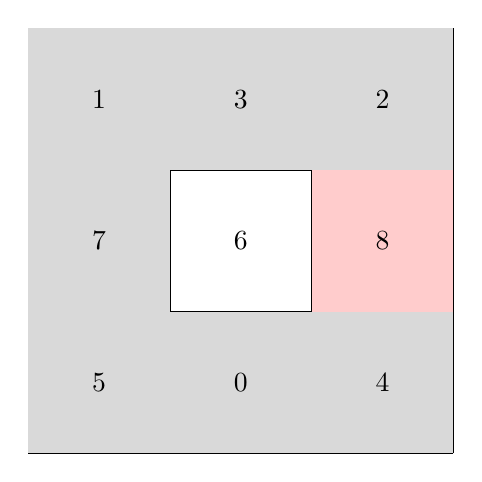
\begin{tikzpicture}[scale=1.8,minimum size=1.8cm]
    \draw (0,0) grid (3,3);
    \node at (0.5,2.5) [fill=gray!30] {1};
    \node at (1.5,2.5) [fill=gray!30] {3};
    \node at (2.5,2.5) [fill=gray!30] {2};
    \node at (0.5,1.5) [fill=gray!30] {7};
    \node at (1.5,1.5) {6};
    \node at (2.5,1.5) [fill=red!20] {8};
    \node at (0.5,0.5) [fill=gray!30] {5};
    \node at (1.5,0.5) [fill=gray!30] {0};
    \node at (2.5,0.5) [fill=gray!30] {4};
\end{tikzpicture}
\caption{\small {The cells that are colored are called the Moore neighborhood of the 6 cell}}
\label{fig:myfigure}
\end{figure}
In Figure \ref{fig:myfigure}, the shaded regions are the Moore neighborhood of the 6 cell located in the middle. As with version 1, the rules of movement was not altered for the prototype and 6 cell can transfer a unit of energy into any one of the grey cells with $\frac{1}{7}$ probability each. \par

\vspace{0.3cm}
\noindent
At this point, I knew the assumption of $\frac{1}{7}$ probability was wrong as in Chemistry, an electron will try to occupy the lowest energy state first rather than going into the higher orbitals. For instance, the way the electron goes toward orbitals is in the following order: ${1s^{2}, 2s^{2}, 2p^{6}, 3s^{2}, 3p^{6}, 4s^{2}, 3d^{10}, 4p^{6}}$. Hence, I needed some method or function that will modify the probabilities of each direction that is dependent on each cell's energy value. \par

\vspace{0.3cm}
\noindent
After some searching and reading articles on this topic, I came across the \href{https://en.wikipedia.org/wiki/Boltzmann_distribution}{Boltzmann factor} which conveniently addressed the problem quite well. The Boltzmann factor is given by: 
\vspace{0.2cm}
\begin{equation}
    \frac{p_{i}}{p_{j}}=e^{\dfrac{\epsilon_{j}-\epsilon_{i}}{kT}}
    \label{modboltz}
\end{equation}
The p terms represent the probability at state i and state j while the $\epsilon$ terms represent the energy at state j and i respectively. At this point, I wasn't exactly sure how to implement the Boltzmann factor to Figure \ref{fig:myfigure}. Since I wanted the simulation to make use of this concept, I decided to modify the Boltzmann factor into: 
\vspace{0.2cm}
\begin{equation}
    p_{j}=e^{\dfrac{8-\epsilon_{j}}{T}}
    \label{eq1}
\end{equation}
In this modified, version $\epsilon_{j}$ represents each cell's energy state within the Moore neighborhood and $p_{j}$ represents the probability that a unit of energy is transferred to that particular cell. \par

\vspace{0.3cm}
\noindent
Using this particular equation we can modify the probability that the 6 cell within Figure \ref{fig:myfigure} transfers its energy to each of the cells shaded grey. To do that we need to compute all of the probabilities and normalize them with a partition function. The partition function is defined as: 
\begin{equation}
    \sum_{j=1}^{\kappa} e^{\frac{8-\epsilon_{j}}{T}}
    \label{eq:2}
\end{equation}
Where $\kappa$ is the number of cells within the neighborhood excluding 8s. So for the picture in Figure \ref{fig:myfigure2}, $\kappa=7$ as we only have 7 "available cells" that the energy from the 6 cell can go to. \par

\vspace{0.3cm}
\noindent
Assuming that T=1, we can then divide each of Boltzmann's factors with \ref{eq:2}. This yields our probabilities of $P=[0.2330, 0.0315,0.0857, 0, 0.0116, 0.6333, 0.0043, 0.0006]$ for the cells labeled: $1, 3, 2, 8, 4, 0, 5, 7$ respectively. This means that there is a 61.6\% chance that the 6 cell within Figure \ref{fig:myfigure2} will send a unit of energy to a 0 cell and a 0.06\% chance that the 6 cell sends a unit of energy towards the 7 cell. \par

\vspace{0.3cm}
\noindent
To better depict the probabilities, I have made the picture below where each of the cell's values has a small text beside it which is the probability that a unit of energy from the 6 cell goes into the other cells. 
\begin{figure}[H]
\centering % center the figure
\begin{tikzpicture}[scale=1.8,minimum size=1.8cm]
    \draw (0,0) grid (3,3);
    \node at (0.5,2.5) [fill=gray!20] {1, \tiny{0.2330}} ;
    \node at (1.5,2.5) [fill=gray!20] {3, \tiny{0.0315}};
    \node at (2.5,2.5) [fill=gray!20] {2, \tiny{0.0857}};
    \node at (0.5,1.5) [fill=gray!20] {7, \tiny{0.0006}};
    \node at (1.5,1.5) {6};
    \node at (2.5,1.5) [fill=red!20] {8, \tiny{0}};
    \node at (0.5,0.5) [fill=gray!20] {5, \tiny{ 0.0043}};
    \node at (1.5,0.5) [fill=gray!20] {0, \tiny{ 0.6333}};
     \node at (2.5,0.5) [fill=gray!20] {4, \tiny{0.0116}};

    \draw [-stealth] ($(1.5,1.5)!0.4!(0.5,2.5)$) -- ($(1.5,1.5)!0.6!(0.5,2.5)$) ;
    \draw [-stealth] ($(1.5,1.5)!0.4!(1.5,2.5)$) -- ($(1.5,1.5)!0.6!(1.5,2.5)$) ;
    \draw [-stealth] ($(1.5,1.5)!0.4!(2.5,2.5)$) -- ($(1.5,1.5)!0.6!(2.5,2.5)$);
    \draw [-stealth] ($(1.5,1.5)!0.4!(0.5,1.5)$) -- ($(1.5,1.5)!0.6!(0.5,1.5)$) ;
    \draw [-stealth] ($(1.5,1.5)!0.4!(2.5,1.5)$) -- ($(1.5,1.5)!0.6!(2.5,1.5)$) ;
    \draw [-stealth] ($(1.5,1.5)!0.4!(0.5,0.5)$) -- ($(1.5,1.5)!0.6!(0.5,0.5)$) ;
    \draw [-stealth] ($(1.5,1.5)!0.4!(1.5,0.5)$) -- ($(1.5,1.5)!0.6!(1.5,0.5)$) ;
    \draw [-stealth] ($(1.5,1.5)!0.4!(2.5,0.5)$) -- ($(1.5,1.5)!0.6!(2.5,0.5)$) ;

\end{tikzpicture}
\caption{\small {Probabilities of each of the cells within the Moore neighborhood of the 6 cell}}
\label{fig:myfigure2}
\end{figure}
We can then model all 8 outcomes depicted by the arrows. In the picture below, I decided on only drawing 2 possible outcomes depicted by arrows with the probabilities associated with them. The rest will be left as an exercise for the reader. 
\begin{figure}[H]
\centering % center the figure
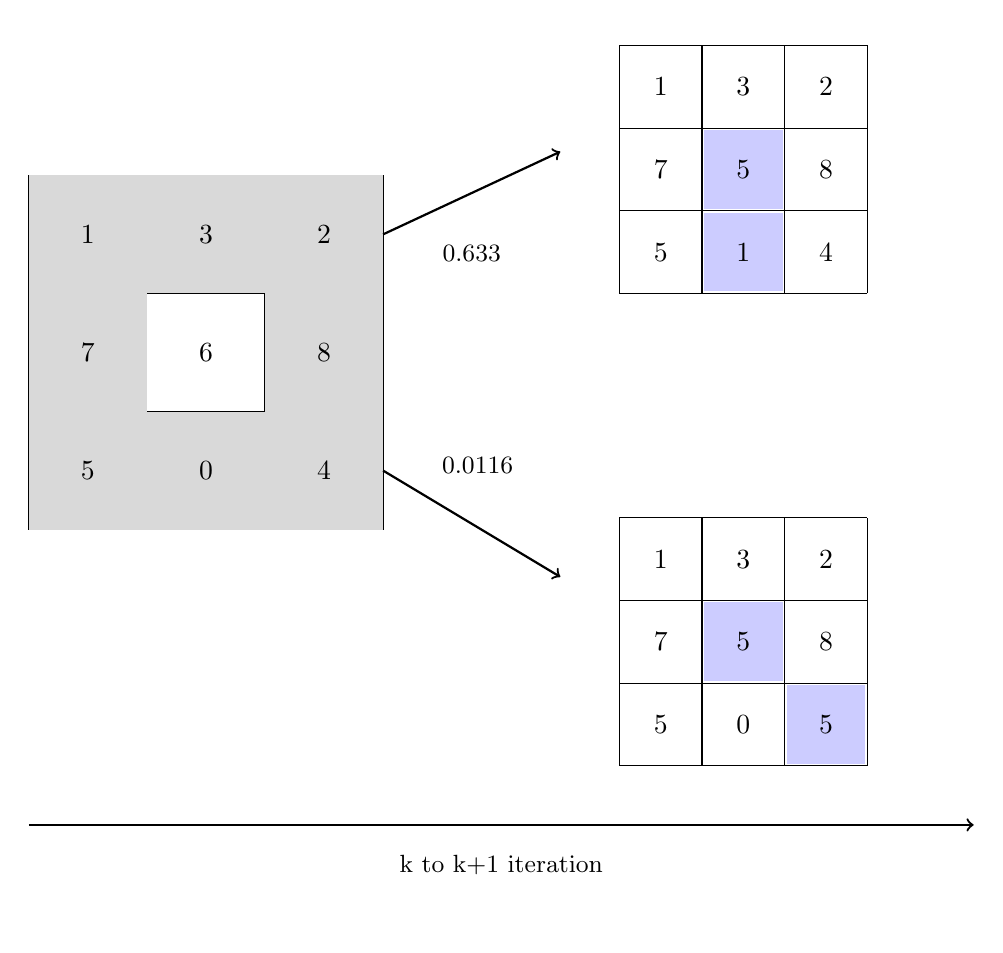
\begin{tikzpicture}[scale=1.5,minimum size=1.5cm]
    \draw (0,0) grid (3,3);
    \node at (0.5,2.5) [fill=gray!30] {1};
    \node at (1.5,2.5) [fill=gray!30] {3};
    \node at (2.5,2.5) [fill=gray!30] {2};
    \node at (0.5,1.5) [fill=gray!30] {7};
    \node at (1.5,1.5) {6};
    \node at (2.5,1.5) [fill=gray!30] {8};
    \node at (0.5,0.5) [fill=gray!30] {5};
    \node at (1.5,0.5) [fill=gray!30] {0};
    \node at (2.5,0.5) [fill=gray!30] {4};
      \draw [->, black, thick] (3.0, 2.5) -- node[below] {\small{0.633}} (4.5, 3.2);
      \draw [->, black, thick] (3.0, 0.5) node[above, shift={(1.2,-0.7)}]{\small{0.0116}} -- (4.5, -0.4);
        \draw [->, black, thick] (0, -2.5) node[below,shift={(6.0,0.25)}]{\small{k to k+1 iteration}} --  (8, -2.5);
         % top branch
        \begin{scope}[shift={(5cm, 2cm)}, scale=0.7]
            \draw (0,0) grid (3,3)   ;
            \node at (0.5,2.5) {1};
            \node at (1.5,2.5) {3};
            \node at (2.5,2.5) {2};
            \node at (0.5,1.5) {7};
            \node at (1.5,1.5) [fill=blue!20, minimum size=1.0cm]{5};
            \node at (2.5,1.5) {8};
            \node at (0.5,0.5) {5};
            \node at (1.5,0.5) [fill=blue!20, minimum size=1.0cm] {1};
            \node at (2.5,0.5) {4};

        \end{scope}
        % Bottom branch
        \begin{scope}[shift={(5cm, -2cm)}, scale=0.7]
            \draw (0,0) grid (3,3)   ;
            \node at (0.5,2.5) {1};
            \node at (1.5,2.5) {3};
            \node at (2.5,2.5) {2};
            \node at (0.5,1.5) {7};
            \node at (1.5,1.5) [fill=blue!20, minimum size=1.0cm]{5};
            \node at (2.5,1.5) {8};
            \node at (0.5,0.5) {5};
            \node at (1.5,0.5) {0};
            \node at (2.5,0.5) [fill=blue!20, minimum size=1.0cm] {5};

        \end{scope}
\end{tikzpicture}
\caption{\small {Possible configurations for the k+1 iteration. Blue cells are the cells whose value changed}}
\label{fig:myfigure3}
\end{figure}
As seen from Figure \ref{fig:myfigure3}, there is a 63.3\% chance that the grid would end up looking like the top and a 1.16\% chance that the grid would look like the bottom in the next iteration. Using this strategy, I can then drift my simulation to be closer to reality.
\pagebreak

\section{Calculating entropy}
Now that a strategy that governs energy movement has been devised, our next task is to find a way to compute entropy. In version 1, a crude method of using bitwise XOR is used. Details on how this is done can be seen within this \href{https://github.com/ShiroHusin/Entropy_Simulation/blob/main/Entropy_Computation.pdf}{document}. However, such a method is not viable when the cells are no longer binary digits. Hence, a new strategy needs to be devised. \par

\vspace{0.3cm}
\noindent
The first step in solving this problem is to look back at the definition of entropy that Ludwig Boltzmann provided. The entropy $S$ is equal to: 
\begin{equation}
    S=k_{b}Ln(\Omega)
    \label{entropy_eq}
\end{equation}
Now the $\Omega$ term is the total number of micro-states or possible configurations that the system can occupy. The challenge is then to find a way to compute $\Omega$. Remembering the \href{https://www.youtube.com/watch?v=mg0hueOyoAw&ab_channel=ParthG}{video} that ParthG made in explaining what entropy is, it became clear that the strategy is to count the number of viable integers combinations that add up a number. \par

\vspace{0.3cm}
\noindent
The technique I decided on is to first, break down the entire square grid into 2x2 sub-matrices. If we let $l$ be equal to the length of the matrix and that $l \in 2\mathbb{Z}$, we would have $\frac{l^2}{4}$ different sub-matrices. In Figure \ref{fig:matrix}, some of the splittings are depicted using arrows and the middle matrix is the grid. Note that the middle matrix is a square matrix, for convenience, it is depicted as a rectangle.

\begin{figure}[H]
  \centering
  \scalebox{1.2}{
    \begin{tikzpicture}[node distance=0.5cm and 0.5cm]
      \node(matrix) {$\begin{bmatrix}
          a_{1,1} & a_{1,2} & \cdots & a_{1,l-1} & a_{1,l} \\
          a_{2,1} & a_{2,2} & \cdots & a_{2,l-2} & a_{2,l} \\
          \vdots  & \vdots  & \vdots & \vdots & \vdots  \\
          a_{l-1,1}& a_{l-1,2} & \ddots &a_{l-1,l-1} & a_{l-1,l}\\
          a_{l,1} & a_{l,2} & \cdots& a_{l,l-1} & a_{l,l}
        \end{bmatrix}$};
        
         \node(submatrix1) [above left=of matrix.north west, xshift=0cm, yshift=1cm] {$\begin{bmatrix}
          a_{1,1} & a_{1,2} \\
          a_{2,1} & a_{2,2}
        \end{bmatrix}$};

         \node(submatrix2) [above right=of matrix.north east, xshift=0cm, yshift=1cm] {$\begin{bmatrix}
          a_{1,l-1} & a_{1,l} \\
          a_{2,l-2} & a_{2,l}
        \end{bmatrix}$};
        
      \node(submatrix3) [below right=of matrix.south west, xshift=-3cm, yshift=-1cm] {$\begin{bmatrix}
          a_{l-1,1} & a_{l-1,2} \\
          a_{l,1} & a_{l,2}
        \end{bmatrix}$};

      \node(submatrix4) [below left=of matrix.south east, xshift=3cm, yshift=-1cm] {$\begin{bmatrix}
          a_{l-1,l-1} & a_{l-1,l} \\
          a_{l,l-1} & a_{l,l}
        \end{bmatrix}$};

        \draw[->, thick] (matrix.north west) -- (submatrix1.south);
        \draw[->, thick] (matrix.north east) -- (submatrix2.south);
      \draw[->, thick] (matrix.south west) -- (submatrix3.north);
      \draw[->, thick] (matrix.south east) -- (submatrix4.north);
    \end{tikzpicture}
  }
  \caption{Submatrix splitting}
  \label{fig:matrix}
\end{figure}

\pagebreak
Now let the grid be called $M$ and its sub-matrices be called $X_{j}$. In this case, $j$ goes from 1 all the way to $\frac{l^2}{4}$. At this point, the next step is $\forall X_{j}$, find the sum of its 4 elements. Now, let the sum of its four elements of each sub-matrix be depicted as $\Phi_{j}$. Remembering the rules of the simulation the sum of its elements or its energy is bounded within: 

$$0\leq \Phi_{j} \leq 32, \;\;\; \Phi_{j} \in \mathbb{Z} $$

Once this is completed, the next step is to find the number of integer combinations of the elements from $X_{j}$, such that its four elements:
\begin{equation}
    a_{j}+b_{j}+c_{j}+d_{j}=\Phi_{j}
    \label{each}
\end{equation}
Where: 
$$a_{j},b_{j},c_{j},d_{j} \in [0,8] \; 	\land \; a_{j},b_{j},c_{j},d_{j} \in \mathbb{Z}$$
\begin{equation}
    \sum_{j=1}^{\frac{l^2}{4}} \Phi_{j} = E
    \label{conservation}
\end{equation}
Now equation \ref{conservation} is the conservation of energy and the simulation is designed such that this is always true. \par

\vspace{0.3cm}
\noindent
Conveniently, there are hundreds of sample codes out there in stack overflow that solve something similar to equation \ref{each}, therefore solving this problem is thankfully not that difficult. The number of possible combinations such that $a_{j}+b_{j}+c_{j}+d_{j}=\Phi_{j}$ is the number of micro-states for each sub-matrix. Lets call this $\omega_{j}$. Some of the calculated values of $\omega_{j}$ corresponding to its $\Phi_{j}$ is shown in the table down below: 
\begin{center}
\begin{tabular}{ |p{4.3cm}|p{3.2cm}|  }
 \hline
Sub-matrix energy ($\Phi_{j}$)& Micro-states ($\omega_{j}$)\\
 \hline
 0 & 1 \\
 1 & 4  \\
 2 & 10 \\
 4 & 35  \\
 6 & 84  \\
 9 & 216  \\
 11 & 324  \\
 14 & 456 \\ 
 16 & 489 \\
\hline
\end{tabular}
\end{center} 
The above table can map $\Phi_{j}$ to its associated $\omega_{j}$ for each sub-matrix $X_{j}$. However, in order to find the total configurations that the grid $M$ can take we have to multiply each of the sub-matrix micro-state where $\Omega$ from equation \ref{entropy_eq} is: 
\begin{equation}
    \Omega=\prod_{j=1}^{\frac{l^2}{4}} \omega_{j}
    \label{Omega}
\end{equation}
For large grids where $l \ge 150$, $\Omega$ becomes a huge number and in some cases, float32 operations in Python may become insufficient. Using the results from equation \ref{Omega} and combining the product rule for logarithms, equation \ref{entropy_eq} can be rewritten as: 
\begin{equation}
    S=k_b\sum_{j=1}^{\frac{l^2}{4}} ln(\omega_{j})
    \label{Total_entropy}
\end{equation}
\vspace{0,3cm}
\noindent
To sum up, while $k\leq I$, and $I$ is the number of iterations. We have:
\begin{figure}[H]
    \centering
    \begin{tikzpicture}[
    SIR/.style={rectangle, draw=red!60, fill=red!5, very thick, minimum size=5mm},
    ]
    %Nodes
    \node[SIR] (Zeroth) {Grid $M$} ;
    \node[SIR]    (First) [below=1.2cm of Zeroth]                              {$\forall a \in M_{k}, \; a \neq 0$};
    \node[SIR]    (Second)    [below=1.2cm of First]       {$F(M_{k},k)$};
    \node[SIR]    (Third)     [below=1.2cm of Second] {$M_{k+1}$};

    \node[SIR] (four) [right=1.2cm of Third]
    {$S(M_{k+1})$};

    \node[SIR] (five) [above=1.2cm of four] {$\omega_{j}$ table} ;

    \node[SIR] (six) [right=1cm of four] {Data-point $(k,S_{k})$} ;
    
    %Lines
    \draw[->, very thick] (Zeroth.south) to node[right] {} (First.north);
    \draw[->, very thick] (First.south)  to node[right] {for each $a$, if $x \sim \mathrm{U}(0,1) <g(c), \;\; U \in \mathbb{R}$} (Second.north);
    \draw[->, very thick] (Second.south)  to node[right] {} (Third.north);
    \draw[->, very thick] (Third.east) to node[right]
    {} (four.west)  ;
    \draw[->, very thick] (five.south) to node[right] {} (four.north) ; 
    \draw[->, very thick] (four.east) to node[right] {} (six.west) ;
    \draw[->, very thick] (Third.west) .. controls  +(left:14mm) and +(left:14mm)   .. node[pos=0.5, left] {$k=k+1$} (Zeroth.west);
    
    \end{tikzpicture}
    \caption{Process or Functional flow diagram}
    \label{fig:my_labels}
\end{figure}
Figure \ref{fig:my_labels} represents a high-level overview of the process steps needed to produce and run the simulation for 1 iteration. $a$ is the elements of the grid/matrix $M$. $U(0,1)$ is a uniform distribution from 0 to 1. $F(M,k)$ is the function responsible for movement, $\omega_{j}$ is the micro-state table, $S(M_{k},k)$ is the entropy function. 

\pagebreak
\chapter{How its made}
\section{How some alcoholic RTDs are made}
As mentioned in section 1.1. Alcoholic RTDs can consist of beverages like Beer, wine, pre-mixed  cocktails, and or alcopops/cider. Let's start with the most popular one which is Beer. 
In general, there are several steps involved in making beer. These steps are shown in the Block-flow diagram (BFD) below:
\begin{figure}[H]
    \centering
    \includegraphics[width=15cm, height=7.5cm]{images/Beer_BFD.png}
    \caption{General Block flow diagram for Beer making}
    \label{fig:beer}
\end{figure}
The steps of the beer-making process can be broken down as follows: 
\begin{enumerate}
  \item \textbf{Malting:} The first step in making beer is to convert raw grains, such as barley, wheat, or rice, into malt, which is the primary ingredient in beer. This process, called malting, involves soaking the grains in water to trick them into thinking that they can germinate. The germination process is stopped by drying the grains.
  \item \textbf{Mashing:} After the grains have been malted, they are then ground into a fine powder called grist. The grist is mixed with hot water in a large vessel called a mash tun, to form a sweet liquid called wort. The wort contains the sugars that will be fermented by the yeast to create alcohol.
  \item \textbf{Boiling: }The wort is then transferred to a large kettle called a brew kettle and brought to a boil. During the boiling process, hops are added to the wort to impart bitterness, flavor, and aroma to the beer. The hops also act as a natural preservative and boiling also sterilize the concentrated wort.
  \item \textbf{Cooling: } After boiling, the wort is cooled quickly to bring it to fermentation temperature.
  \item \textbf{Fermentation: }The cooled wort is then transferred to a fermentation tank and yeast is added to start the fermentation process. Yeast converts the sugars in the wort into alcohol and carbon dioxide, which will create the characteristic effervescence of the beer.
  \item \textbf{Aging: }After fermentation, the beer is typically aged for a period of time in order to allow the flavors to develop and to clarify the beer.
  \item \textbf{Filtering: }The beer is then filtered to remove any remaining yeast or sediment, in order to make the beer clear.
  \item \textbf{Carbonation and packaging: }After filtering, the beer is carbonated, either naturally by introducing sugar or additional yeast, or by injecting carbon dioxide under pressure. The beer is then packaged into bottles, cans, or kegs, and is ready to be shipped to the consumer. 
\end{enumerate}
Another prominent alcoholic RTD that is commonly brought is wine. This process of making wine can vary depending on the type of wine but in general wine-making follows these steps: 
\begin{enumerate}
  \item \textbf{Harvest:} The first step in making wine is to harvest the grapes when they are at their peak of ripeness. This is typically done by hand, although mechanization is also used in some regions.
  \item \textbf{Crusing and pressing:} After the grapes are harvested, they are then crushed and pressed to extract the juice. During crushing, the grapes are broken down to release the juice. Pressing is used to extract more juice from the grapes and sometimes remove the skins. This process will vary depending on whether red, white or rosé wine is being made.
  \item \textbf{Fermentation: }The juice, called must, is then transferred to fermentation tanks. Yeast is added to start the fermentation process where the juice is converted into alcohol and carbon dioxide. The fermentation process can vary depending on the type of grape and the desired final product.
  \item \textbf{Clarification: }After fermentation, the wine is clarified to remove any remaining solids. This process can include techniques such as racking, fining, and filtration.
  \item \textbf{Aging: }After clarification, the wine is aged in oak barrels or stainless steel tanks. During this time, the wine develops its unique flavors and aromas.
  \item \textbf{Blending and packaging: }After aging, the winemaker will taste the wine and decide which barrels or tanks to blend together to create the final product. The wine is then bottled, corked, and sealed, ready for shipment and consumption.
\end{enumerate}
\section{How some non-alcoholic RTDs are made}
As mentioned in section 1.1, non-alcoholic RTDs can consist of Juice drinks, Tea or Coffee, and Carbonated drinks. It can also range towards more exotic RTDs like sports drinks, Kombucha, Diary products, or packaged coconut water.  \par

\vspace{0.3cm}
To make an RTD juice drink,  one can select from a huge repertoire of fruits such as mango, guava, apple, watermelon, and many others. However, the general block flow diagram of making juice drinks is: 
\begin{figure}[H]
    \centering
    \includegraphics[width=12cm, height=10cm]{images/Juice_BFD.png}
    \caption{General Block flow diagram for juice RTDs}
    \label{fig:juice}
\end{figure}
Breaking down each step into greater detail: \begin{enumerate}
  \item \textbf{Washing and dicing: } The first step in making juice RTDs is to extract the pulp and the fruit juice by dicing and pressing it.
  \item \textbf{Pulping: } The fruit pulp, the juice, and the fibers are collected. Depending on regulations, the fruit component has to be larger than a certain percentage. 
  \item \textbf{Filtering: }Prior to filtering, the fruit juice extract is added with sugar syrup like sucrose to assist in providing flavor. Filtering of juice is done to remove the solids that are present within the fruit extract. 
  \item \textbf{Homogenization: } After filtration, the fruit extract is homogenized to make an even distribution of total dissolved solids and liquids within the product. 
  \item \textbf{Mixing: }Prior to mixing, the fruit is added with preservatives and or color or citric acid. Preservatives are added so that its shelf life is prolonged and acid is used to produce a balance between sugars and acid and make a consistent flavor.
  \item \textbf{Sterilization: }After mixing is done, the mixture is sterilized to ensure that no potential bacteria or fungi grow within the product. Some companies might use flash sterilization and some don't. To each their own.
  \item \textbf{Packaging: } Finally, the product is then packaged in sterilized bottles and ready to be shipped. 
\end{enumerate}
Finally, seeing that Process Partners also do Kombucha a tea drink made from fermented tea leaves. I decided to make some sort of research on the manufacture of this RTD. Essentially, Kombucha is a fermented tea drink that is made by combining tea, sugar, and a symbiotic culture of bacteria and yeast, also known as a SCOBY (Symbiotic Culture Of Bacteria and Yeast) which creates a fermentation process that results in the formation of a probiotic beverage. The general process flow for making kombucha is as follows:
\begin{enumerate}
  \item \textbf{Tea brewing: } The first step in making kombucha is to brew the tea. This is typically done by steeping black or green tea leaves in hot water for a period of time, depending on the desired strength of the tea.
  \item \textbf{Sweetening: } After the tea has been brewed, sugar is added to the tea to feed the yeast culture. The amount of sugar added will depend on the desired final product and the length of fermentation.
  \item \textbf{Cooling: }The tea is then cooled to room temperature to ensure that it is at a safe temperature to add the starter culture 
  \item \textbf{SCOBY addition: } The cooled tea is then poured into a fermenting container and the SCOBY culture is added. The SCOBY culture contains the symbiotic bacteria and yeast that will ferment the tea and create kombucha.
  \item \textbf{Fermentation: }The mixture is then left to ferment for a period of time, depending on the desired final product and the length of fermentation. The length of time depends on factors such as temperature, pH level, and the type of yeast and bacteria used.
  \item \textbf{Flavorings: }After fermentation, the kombucha can be flavored with different fruits, herbs, or spices.
  \item \textbf{Packaging: }The Kombucha is then bottled in sterilized cans or plastic bottles.
\end{enumerate}
\pagebreak
\section{Differing process flows}
\subsection{Kombucha}
The above BFD's present a general process flow for making Beer, wine, juice, and Kombucha. However, each region might have different ways to make the final RTD. \par

\vspace{0,3cm}
If we take Kombucha as an example, the tea that is used to make Kombucha is different for different parts of the world. To my knowledge, it seems that Black tea is often the main ingredient used to make Kombucha but in China, green tea is often used to make Kombucha. \par

\vspace{0,3cm}
In the sweetening process for Kombucha, some regions and companies associated with those regions might use honey, maple syrup, or jaggery (cane sugar) to sweeten the drink instead of normal white sugar. In terms of the flavorings process, local regions especially in southeast Asia might use local ingredients such as ginger or lemongrass to cater with the local demand. \par

\vspace{0,3cm}
Likewise, GDP can also play a role in predicting what sort of method is in use. A country/sector with lower GDP might not have the same process flow for making kombucha but instead, the process might be entirely homemade. Just like winemaking, some regions might use physical labor rather than a mechanical press or machinery to press grapes or brew the tea. \par

\vspace{0,3cm}
\subsection{Beer}
In terms of beer making, the basic process of producing beer remains the same. That is it follows the steps of Malting, Mashing, Boiling, and Fermenting. \par

\vspace{0,3cm}
However, for different parts of world beer making differs in the ingredients used. In Germany, under the Reinheitsgebot law, which was introduced by by Duke Wilhelm IV of Bavaria in the year 1516, is still enforced today. This means that only Barley, Hops, yeast and water can only be used to make German beer. On the other hand, grains such as wheat, rice, oat or rye are commonly found in other beer brewing process. \par

\vspace{0,3cm}
Some people might add local products into Beer making. Such as adding fruits or spices into the final product. The timing on when these things are added are not exact and depends on the manufacturer's flavor profile. Some add it during the fermentation phase, which allows the yeast to interact with the spices and fruits creating a deep complex flavor, others add it at the end of the beer making process. \par

\vspace{0.3cm}
There are other notable examples of differences of the beer making process. For instance, in Africa beer is made from locally sourced ingredients such as millet, sorghum and maize instead of the traditional barley and hops. In Asia, Beer is often made with rice producing rice beer with a highly different flavor. 

\subsection{Juice RTDs}
Just like with the manufacture of Kombucha or beer. The process of making juice-ready-to-drink (RTD) beverages remains generally the same. That is the process of sourcing the juice, cleaning, cutting, pressing, pasteurizing, packaging and shipping is similar across the world. However, depending on region and local taste, the process shown in \ref{fig:juice} might differ slightly. \par

\vspace{0.3cm}
For instance, in countries where sugar cane grows such as southeast Asia, the Caribbeans or Africa a concentrated sweet dark liquid of boiling sugarcane juice might be used instead of sugar syrup. Additionally, different regions may have different ways of pasteurising its final product, some might employ normal pasteurisation while others might use flash pasteurisation where the stream is brought to a higher temperature but for a much shorter length of time. This flash pasteurisation process is typically used for easily perishable products; products that spoils easily. 
\pagebreak

\section{A possible PFD for beer making}
\begin{figure}[H]
    \centering
    \includegraphics[width=20cm, height=15cm,angle=-90]{images/Beer_PFD.jpg}
    \caption{General PFD for Beer making}
    \label{fig:beer_PFD}
\end{figure}
\pagebreak

Tables that explain ambiguous stream in more detail is shown down below:
\begin{center}
\begin{tabular}{ |p{3cm}||p{3cm}||  }
 \hline
 \multicolumn{2}{|c|}{\textbf{Stream description}} \\
 \hline
Stream number& Description\\
 \hline
3 & Grist\\
8 & Mash tun\\
11& Wort\\
14& Fermentation mixture\\
17& Beer filtrate\\
18& Packaged RTD beer\\
 \hline
\end{tabular}
\end{center}


\pagebreak
\chapter{Conclusion}
\noindent
Research on RTD drinks were made to answer the question on how RTD drinks are made in different parts of the world and what sort of RTD drinks are available. \par

\vspace{0.3cm}
\noindent
The RTD category can be mainly broken down into 2 sections alcoholic and non-alcoholic RTDs. Alcoholic RTDs include: Beer, Wine, Alcopolps, and cider. Non-alcoholic RTDs include: Juice drinks, Tea and Coffee beverages, Carbonated drinks, Sports drinks, Kombucha, Diary products and many more.  \par

\vspace{0.3cm}
\noindent
Answering the question on what sort of RTD drinks are available throughout the world requires a data-driven approach where the alcohol consumption per capita per year and GDP per capita are used as proxy measurements on the demand of RTDs. Countries with low levels of alcohol consumption per capita is unlikely to have a large repertoire of alcoholic RTDs. Similarly, countries with low GDP per capita is probably unvaried in its offerings of different types of non-alcoholic RTDs. \par

\vspace{0.3cm}
\noindent
The Process of making RTDs generally follow the same pattern. However, regional demand and law might dictate what sort of ingredients are used. For example, in Germany, only barley, hops, water and yeast are allowed for beer making. In other parts of the world, the Barley can be mixed with rice or other grains such as sorghum, maize or rye. 

\pagebreak
\bibliographystyle{IEEEtran} 
\bibliography{Reference}


\end{document}
